% This file was created with tikzplotlib v0.9.15.
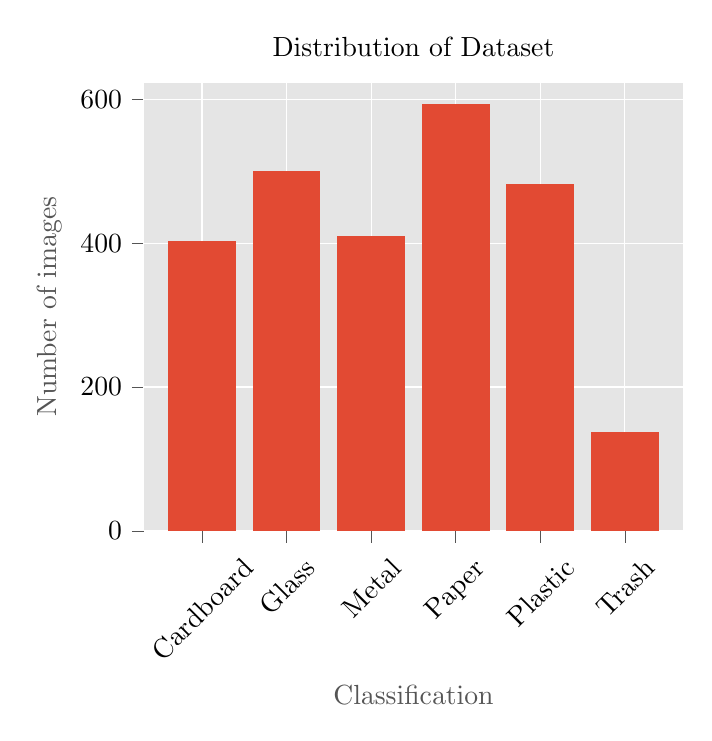
\begin{tikzpicture}

\definecolor{color0}{rgb}{0.886274509803922,0.290196078431373,0.2}

\begin{axis}[
axis background/.style={fill=white!89.8039215686275!black},
axis line style={white},
tick align=outside,
tick pos=left,
title={Distribution of Dataset},
x grid style={white},
xlabel=\textcolor{white!33.3333333333333!black}{Classification},
xmajorgrids,
xmin=-0.69, xmax=5.69,
xtick style={color=white!33.3333333333333!black},
xtick={0,1,2,3,4,5},
xticklabel style={rotate=45.0},
xticklabels={Cardboard,Glass,Metal,Paper,Plastic,Trash},
y grid style={white},
ylabel=\textcolor{white!33.3333333333333!black}{Number of images},
ymajorgrids,
ymin=0, ymax=623.7,
ytick style={color=white!33.3333333333333!black}
]
\draw[draw=none,fill=color0,very thin] (axis cs:-0.4,0) rectangle (axis cs:0.4,403);
\draw[draw=none,fill=color0,very thin] (axis cs:0.6,0) rectangle (axis cs:1.4,501);
\draw[draw=none,fill=color0,very thin] (axis cs:1.6,0) rectangle (axis cs:2.4,410);
\draw[draw=none,fill=color0,very thin] (axis cs:2.6,0) rectangle (axis cs:3.4,594);
\draw[draw=none,fill=color0,very thin] (axis cs:3.6,0) rectangle (axis cs:4.4,482);
\draw[draw=none,fill=color0,very thin] (axis cs:4.6,0) rectangle (axis cs:5.4,137);
\end{axis}

\end{tikzpicture}
